%% LyX 1.1 created this file.  For more info, see http://www.lyx.org/.
%% Do not edit unless you really know what you are doing.
\documentclass[prb,aps,twocolumn]{revtex4}

\usepackage{graphicx}
\usepackage{amsfonts}
\usepackage{amsmath}
\usepackage{bm}
\usepackage{alltt}
\usepackage{dcolumn} 
\usepackage{amsmath} 
\usepackage{graphicx}
\makeatletter 
\makeatother

\begin{document}

\title{\textbf{Linear scaling computation of the Fock matrix VI. Gaussian
orbital methods for simulation of periodic systems}}


\author{C.J. Tymczak}
\author{Matt Challacombe}

\affiliation{Theoretical Division, Los Alamos National Laboratory, Los Alamos,
New Mexico 87545 }

\date{\today}

\begin{abstract}
Periodic boundary conditions have been implemented in the linear scaling
Quantum Chemistry code \textbf{MondoSCF}. For the two-electron Coulomb
matrix, this has been achieved with an exact multipole expansion of
the long range Coulomb field. This yields a spherically summed boundary
condition that is easily transformed to Ewald boundary conditions.
In order to achieve linear scaling of the local Coulomb field, a Quantum
Chemical Tree Code (QCTC) is used. Periodic boundary conditions have
also been incorporated into calculations of the local exchange-correlation
matrix and the exact-exchange matrix. A Hierarchical Cubature (HiCu),
pure Cartesian adaptive grid is used for the local exchange-correlation
matrix. This method achieves linear scaling through the use of advanced
data structures (k-d trees) that maximally exploits locality of the
density. Finally, the current capabilities of MondoSCF for large condensed
phases will be demonstrated.
\end{abstract}

\maketitle

\section{INTRODUCTION}

When simulating bulk behavior in solids or liquids, Periodic Boundary
Conditions (PBC) are often essential to employ \cite{Allen90}. Therefore,
we have implemented Periodic boundary conditions into the linear scaling
Quantum Chemistry code \textbf{MondoSCF} 
\cite{Challacombe96,Challacombe97,Challacombe99}.
For the one electron matrix this has been achieved by a re-summation
over periodic cell images, which because of locality leads to an efficient
calculation of the one electron matrices. For the two electron matrices
various methods are employed. For the two-electron Coulomb matrix,
we achieve this via an exact multipole expansion of the long range
Coulomb field \cite{White94,Challacombe97b}. This yields a spherically
summed boundary condition that is easily transformed to Ewald boundary
condition \cite{Redlack72,Redlack75}. In order to achieve linear
scaling of the local Coulomb field, a Quantum Chemical Tree Code (QCTC)
is used {[}ref{]}. For the calculations of the local exchange-correlation
matrix, a Hierarchical Cubature (HiCu), pure Cartesian adaptive grid
is used. This method achieves linear scaling through the use of advanced
data structures (k-d trees) that maximally exploits locality of the
density, and allows for an efficient treatment of the periodic effects
{[}ref{]}. And finally we exploit the locality of the basis functions
to calculate the exact exchange matrix. 

To demonstrate the capabilities of MondoSCF, we show results for three
test condensed phases, Sodium Chloride, Magnesium Oxide and Carbon
in the diamond structure. We then compare these results to the periodic
Gaussian code \textbf{Crystal98} {[}ref{]}. \textbf{}Next we demonstrate
the utility of the code on very large systems such as zeolite. Finally
we give some conclusion concerning the accuracy and utility of MondoSCF
and future research directions.

\section{One-Electron Matrices}

The first step in including periodic boundary conditions into our
linear scaling code is to determine the minimal modifications to the
one-electron integrals needed to obtain this. We incorporate periodic
boundary conditions into our linear scaling method by modifying the
integrals. Consider the non-periodic overlap matrix

\begin{equation}
\label{Sab_norm}
S_{ab}=\int _{V_{\infty }}\, d{\mathbf{r}}\, \phi _{a}({\mathbf{r}})\phi _{b}
({\mathbf{r}})
\end{equation}
 where \( \{\phi _{a}(x),\phi _{b}(x)\} \) are the atomic orbitals
(LCAO) at atom \( a \) and atom \( b \) and \( V_{\infty } \) is
the integration over all space. In the periodic case this is replaced
by {[}ref{]},

\begin{equation}
\label{Sab_pbc1}
S_{ab}^{PBC}=\sum _{\mathbf{R},\mathbf{R}'}\int _{V_{cell}}\, d{\mathbf{r}}\, 
\phi _{a}({\mathbf{r}+\mathbf{R}})\phi _{b}({\mathbf{r}+\mathbf{R}'})
\end{equation}
where, \( V_{cell} \) is the integration over the simulation cell,
and \( \{\mathbf{R},\mathbf{R}'\} \) are the brava lattice vectors,
this is illustrated in figure \ref{figure: SimCell}, where \( \left\{ {\mathbf{a},
\mathbf{b},\mathbf{c}}\right\}  \)
are the primitive lattice vectors. Because of the locality of the
atomic orbitals, we can remove the double sum over lattice vectors
to get

\begin{equation}
\label{Sab_pbc2}
S_{ab}^{PBC}=\sum _{\mathbf{R}}\int _{V_{\infty }}\, d{\mathbf{r}}\, \phi _{a}
({\mathbf{r}})\phi _{b}({\mathbf{r}+\mathbf{R}})
\end{equation}
We will use this Periodic Localization Transformation (PLT) repeatedly
in what follows. Let us present some useful definitions:

\begin{equation}
\label{rho_loc}
\rho ^{loc}({\mathbf{r}})=\sum _{\mathbf{R}}\sum _{ab}{\mathbf{P}}_{ab}\phi _{a}
({\mathbf{r}})\phi _{b}({\mathbf{r}+\mathbf{R}})
\end{equation}
and because of periodicity,

\begin{equation}
\label{rho_pbc}
\rho ^{PBC}({\mathbf{r}})=\sum _{\mathbf{R}}\, \rho ^{loc}({\mathbf{r}+\mathbf{R}})
\end{equation}
We also define:\begin{equation}
\label{rho_loc_ab}
\rho _{ab}^{loc}({\mathbf{r}})=\sum _{\mathbf{R}}\phi _{a}({\mathbf{r}})\phi _{b}
({\mathbf{r}+\mathbf{R}})
\end{equation}


\begin{equation}
\label{rho_pbc_ab}
\rho _{ab}^{PBC}({\mathbf{r}})=\sum _{\mathbf{R}}\, \rho _{ab}^{loc}({\mathbf{r}+
\mathbf{R}})
\end{equation}
Which allows us to rewrite the overlap matrix as

\begin{equation}
\label{Sab_pbc_3}
S_{ab}^{PBC}=\int _{V_{\infty }}\, d{\mathbf{r}}\, \rho ^{loc}_{ab}({\mathbf{r}}).
\end{equation}
Finally, we can rewrite the kinetic energy matrix as

\begin{equation}
\label{Tab_pbc}
T^{PBC}_{ab}=-\frac{1}{2}\sum _{\mathbf{R}}\int _{V_{\infty }}\, d{\mathbf{r}}\, 
\phi _{a}({\mathbf{r}+\mathbf{R}})\nabla ^{2}\phi _{b}({\mathbf{r}})
\end{equation}



\section{The Two-Electron matrices}


\subsection{The Coulomb matrix}

In order to calculate the coulomb matrix efficiently, we transform
the two-electron Coulomb integrals into integrals over all space with
local distributions via PLT transformation and equations (\ref{rho_pbc})
and (\ref{rho_pbc_ab}) {[}ref{]}, 

\begin{equation}
J_{ab}^{PBC}  =  \frac{1}{2}\int _{V_{cell}}\int _{V_{\infty }}\, d{\mathbf{r}}\, 
d{\mathbf{r}'}\frac{\rho _{ab}^{PBC}\left( {\mathbf{r}}\right) \: 
\rho ^{PBC}\left( \mathbf{r}'\right) }{\left| \mathbf{r}-\mathbf{r}'\right| }
\nonumber
\end{equation}
\begin{equation}
\,\,\,\,\,\,\,\,\,\,\,
\,\,\,\,\,\,\,\,\,\,\,
\,\,\,
= \frac{1}{2}\sum _{\mathbf{R}'}\int _{V_{\infty }}\int _{V_{\infty }}\, 
d{\mathbf{r}}\, d{\mathbf{r}'}\frac{\rho _{ab}^{loc}\left( {\mathbf{r}}\right) \: 
\rho ^{loc}\left( {\mathbf{r}'}+{\mathbf{R}'}\right) }{\left| \mathbf{r}-\mathbf{r}'
\right| }
\\
\label{Jab_pbc2} 
\end{equation}
However, this is still a long ranged integral. Let us separate the
Coulomb integral into three pieces 
\begin{equation}
J_{ab}^{PBC}=J_{ab}^{QCTC}+J_{ab}^{PFF}+J_{ab}^{EC}
\label{Jab_sum}
\end{equation}
where 
\begin{equation}
J_{ab}^{QCTC}=\frac{1}{2}\sum _{{\mathbf{R}'}\in V_{in}}\, \int _{V_{\infty }}\, 
\int _{V_{\infty }}\, d{\mathbf{r}}\, d{\mathbf{r}'}\frac{\rho ^{loc}_{ab}\left( {\mathbf{r}}\right)
 \: \rho ^{loc}\left( {\mathbf{r}'+\mathbf{R}'}\right) }{\left| \mathbf{r}-\mathbf{r}'\right| }
\label{Jqctc}
\end{equation}
%
\begin{equation}
J_{ab}^{PFF}=\frac{1}{2}\sum _{{\mathbf{R}'}\in V_{out}}\, \int _{V_{\infty }}
\, \int _{V_{\infty }}\, d{\mathbf{r}}\, d{\mathbf{r}'}\frac{\rho _{ab}^{loc}\left( {\mathbf{r}}\right) 
\: \rho ^{loc}\left( {\mathbf{r}'+\mathbf{R}'}\right) }{\left| \mathbf{r}-\mathbf{r}'\right| }
\label{Jpff}
\end{equation}
%
\begin{equation}
J_{ab}^{EC}=\frac{1}{2}\sum _{{\mathbf{R}'}\in S_{\infty }}\, \int _{V_{\infty }}\, \int _{S_{\infty }}
\, d{\mathbf{r}}\, d{\mathbf{r}'}\frac{\rho _{ab}^{loc}\left( {\mathbf{r}}\right) \: 
\rho ^{loc}\left( {\mathbf{r}'+\mathbf{R}'}\right) }{\left| \mathbf{r}-\mathbf{r}'\right| }
\label{Jec}
\end{equation}
and \( V_{in} \) is the volume which contains the inner cells, \( V_{\infty } \)
is the total volume, \(V_{out}\) is the total volume minus \( V_{in} \), and \( S_{\infty } \) is 
the surface at infinity which contributes a shape dependent potential to the center cell.
This is depicted in figure \ref{figure:ReplicateCells}. Let us now
define and discuss the calculation of each terms.


\subsubsection{The Quantum Chemical Tree Code: The direct Coulomb matrix}

In-order to achieve linear scaling, we use a quantum chemical tree
code {[}ref{]} to compute the integrals in equation (\ref{Jqctc}).
This requires that we replace the integrals in equation (\ref{Jqctc})
with the approximate spherical multipole expansion to order \( L \)
and \( L' \),
%
\begin{equation}
\frac{1}{2}\sum _{{\mathbf{R}'}\in V_{in}}\int _{V_{\infty }}\, d{\mathbf{r}}\, 
d{\mathbf{r}'}\frac{\rho _{ab}^{loc}\left( {\mathbf{r}}\right) \: \rho ^{loc}
\left( {\mathbf{r}'+\mathbf{R}'}\right) }{\left| \mathbf{r}-\mathbf{r}'\right| }
\qquad \qquad \qquad \qquad \qquad \qquad \qquad \qquad \qquad \qquad 
\nonumber
\end{equation}
%
\begin{equation}
\approx \frac{1}{2}\sum _{\mathbf{R}}\sum _{\mathbf{R}'\in V_{in}}
\sum _{\left\langle i\right\rangle }\int _{V_{\infty }}\, d{\mathbf{r}}\, 
d{\mathbf{r}'}\frac{\phi _{a}({\mathbf{r}})\phi _{b}({\mathbf{r}+\mathbf{R}})\: 
\Lambda ^{\left\langle i\right\rangle }\left( {\mathbf{r}'+\mathbf{R}'}\right) }
{\left| \mathbf{r}-\mathbf{r}'\right| }\qquad \qquad \qquad 
\nonumber
\end{equation}
%
\begin{equation}
\qquad\qquad+\frac{1}{2}\sum _{\mathbf{R}}\sum _{\mathbf{R}'\in V_{in}}\sum _{l=0}^{L}\, \sum _{l'=0}^{L'}\, 
\sum _{m=-l}^{l}\, \sum _{m'=-l'}^{l'}\qquad \qquad \qquad \qquad \qquad  
\nonumber
\end{equation}
%
\begin{equation}
\left( -1\right) ^{l}\, {\cal O}^{m}_{l}\left[ \rho _{ab};\mathbf{Q}(\mathbf{R})\right] 
\, M_{l+l'}^{m+m'}[\mathbf{Q}-\mathbf{P}-\mathbf{R}']\, {\cal O}_{l}^{m}[\widetilde{\Lambda }^{\left\langle 
j\right\rangle };\mathbf{P}]
\label{QCTC}
\end{equation}
%
where
\begin{equation}
\label{sp_rho_loc}
O_{l}^{m}\left[ \rho ;\mathbf{P}\right] =\int _{V_{\infty }}\, d\mathbf{r}\, \widehat{O}_{l}^{m}
\left[ \mathbf{r}-\mathbf{P}\right] \, \rho \left( \mathbf{r}\right) 
\end{equation}
\( \Lambda ^{\left\langle i\right\rangle } \) are the set of distributions
of the local density which overlap \( \phi _{a}({\mathbf{r}})\phi _{b}({\mathbf{r}+\mathbf{R}}) \)
(therefore these integrals must be done explicitly) , \( \mathbf{Q}(\mathbf{R}) \)
is the center of the distribution \( \phi _{a}({\mathbf{r}})\phi _{b}({\mathbf{r}+\mathbf{R}}) \),
\( \widetilde{\Lambda }^{\left\langle j\right\rangle } \)are the
set of distributions of the local density which do not overlap \( \phi _{a}({\mathbf{r}})\phi _{b}
({\mathbf{r}+\mathbf{R}}) \),
are organized on a tree, allow us to achieve linear scaling, and are
the multipoles of these densities. The multipole operators are are
defined as

\begin{eqnarray}
\widehat{O}_{l}^{m}\left[ {\mathbf{R}}\right]  & = & \frac{\left| {\mathbf{R}}\right| ^{l}P_{l}^{m}
\left( \cos \left( \theta _{\mathbf{R}}\right) \right) \, e^{-im\phi _{\mathbf{R}}}}{\left( l+m\right) !}
\begin{array}{c}
\\

\end{array}\label{sp_mult_O} \\
M_{l}^{m}\left[ {\mathbf{R}}\right]  & = & \frac{\left( l-m\right) !\, P_{l}^{m}\left( \cos \left( 
\theta _{\mathbf{R}}\right) \right) \, e^{-im\phi _{\mathbf{R}}}}{\left| {\mathbf{R}}\right| ^{l+1}}
\begin{array}{c}
\\

\end{array}\label{sp_mult_M} 
\end{eqnarray}
 In Appendix A we give a short derivation of the overlap, or penetration
error bound that we use and a more detail analysis will be given in
reference {[}ref{]}. In Appendix B we also give a derivation of the
multipole error bound that we use, where also a more detailed analysis
will be given in reference {[}ref{]}. 


\subsubsection{The Periodic Far Field Coulomb matrix}

To obtain the periodic far field correction to the matrix elements
we replace the integral in equation (\ref{Jpff}) with the multipole
sum {[}ref{]}
%
\begin{eqnarray}
J_{ab}^{PFF} &=& \frac{1}{2}\sum _{{\mathbf{R}'}\in V_{\infty }-V_{in}}\, \int _{V_{\infty }}
\, d{\mathbf{x}}\, d{\mathbf{x}'}\frac{\rho _{ab}^{loc}\left( {\mathbf{x}}\right) \: \rho ^{loc}
\left( {\mathbf{x}'+\mathbf{R}'}\right) }{\left| \mathbf{x}-\mathbf{x}'\right| } 
\nonumber\\
&=& \frac{1}{2}\sum _{{\mathbf{R}}\in V_{\infty }-V_{in}}\, \sum _{l=0}^{L}\, 
\sum _{l'=0}^{L'}\, \sum _{m=-l}^{l}\, \sum _{m'=-l'}^{l'}
\nonumber\\
 & & \left( -1\right) ^{l}\, {\cal O}_{l}^{m}[\rho _{ab}^{loc};\mathbf{R}_{0}]
\, M_{l+l'}^{m+m'}[\mathbf{R}]\, {\cal O}_{l'}^{m'}[\rho ^{loc};\mathbf{R}_{0}]
\nonumber\\
& &\label{Jpff_2} 
\end{eqnarray}
%
where \( \mathbf{R}_{0} \) is an arbitrary point in the simulation
cell (usually the center of the cell). Let us define
\begin{equation}
\label{ScriptM}
{\cal M}_{l}^{m}=\sum _{{\mathbf{R}'}\in V_{\infty }-V_{in}}\, M_{l}^{m}[\mathbf{R}]
\end{equation}
Which allow us to rewrite
%
\begin{eqnarray}
J_{ab}^{PFF} &=&\frac{1}{2}\sum _{l=0}^{L}\, \sum _{l'=0}^{L'}\, \sum _{m=-l}^{l}\, \sum _{m'=-l'}^{l'}
\nonumber\\
& & \left( -1\right) ^{l}\, {\cal O}_{l}^{m}[\rho _{ab}^{loc};\mathbf{R}_{0}]\,
 {\cal M}_{l+l'}^{m+m'}\, {\cal O}_{l'}^{m'}[\rho ^{loc};\mathbf{R}_{0}]
\nonumber\\
\label{sp_jpff_2}
\end{eqnarray}
%
For \( l=1 \) and \( 2 \) equation (\ref{ScriptM}) is a conditional
summation. In Appendix C we describe an efficient method which allow
us calculate these conditional summations. The only task remaining
is to determine the region of the inner box summation or the multipole
order \( L \) which we have to expand to. Using equation (\ref{B30})
from Appendix B we obtain for the error bound
\begin{equation}
\label{Rmax}
\tau \leq \frac{C_{\rho }\left| \mathbf{d}_{max}\right| ^{L+1}}{\left| \mathbf{R}_{max}
\right| ^{L+1}\left| \left| \mathbf{R}_{max}\right| -2\left| \mathbf{d}_{max}\right| \right| }
\end{equation}
where we are assuming a \( l_{0}=0 \) distribution of unit weight,
and \( \mathbf{R}_{max} \) is the distance to the nearest cell in
the sum in equation (\ref{ScriptM}). 

In the next section we describe the corrections to the Coulomb matrix
which allows us to obtain Ewald boundary conditions in order to obtain
translational invariance in the matrix elements, and also allows us
to compare directly to \textbf{Crystal98}. Figure \ref{figure: ErrorPFF}
shows the error of the energy as we increase \( L \) from \( 4 \)
to \( 64 \) for two different inner cell sums for a classical system
of \( 64 \) water molecules. As can be seen we obtain very rapid
convergence.


\subsubsection{The Ewald Correction matrix}

The correction to the Coulomb matrix is strongly dependent on how
the periodic multipole tensor is summed. If the matrix is a spherically
ordered lattice sum, then the connection between the spherically ordered
potential and the Ewald potential is \cite{Redlack72}, 
\begin{equation}
\Phi _{Ew}\left( \mathbf{x}\right) =\Phi _{ss}\left( \mathbf{x}\right) -\frac{4\pi }{3}
{\left( \mathbf{x}-\mathbf{R}_{0}\right) \cdot \mathbf{D}}+\frac{2\pi }{3}Q
\label{EW_pot}
\end{equation}
%
in terms of the matrix elements of \( J_{ab}^{PBC} \) this gives
the corrections
\begin{eqnarray}
J_{ab}^{EC} & = & \int _{V_{\infty }}\, d{\mathbf{x}}\, \rho ^{loc}_{ab}\left( {\mathbf{x}}
\right) \left\{ \frac{2\pi }{3}Q-\frac{4\pi }{3}\left( \mathbf{x}-\mathbf{R}_{0}\right) \cdot 
\mathbf{D}\right\}
\nonumber\\
 & = & \frac{2\pi }{3}Q\, S_{ab}^{PBC}-\frac{4\pi }{3}\mathbf{d}_{ab}\cdot \mathbf{D}
\nonumber\\
\label{Jab_ec_2} 
\end{eqnarray}
where
%
\begin{eqnarray}
{\mathbf{d}}_{ab} & = & \int _{V_{\infty }}\, d{\mathbf{x}}\, \left( \mathbf{x}-\mathbf{R}_{0}\right)
 \rho ^{loc}_{ab}\left( \mathbf{x}\right)
\label{dab} \\
{\mathbf{D}} & = & \int _{V_{\infty }}\, d{\mathbf{x}}\, \left( \mathbf{x}-\mathbf{R}_{0}\right) 
\rho ^{loc}\left( \mathbf{x}\right) 
\label{D} \\
Q & = & \int _{V_{\infty }}\, d{\mathbf{x}}\, \left( \mathbf{x}-\mathbf{R}_{0}\right) ^{2}
\rho ^{loc}\left( \mathbf{x}\right) 
\label{Q} 
\end{eqnarray}
are the dipole and quadrapole moments. In appendix D we give a short
derivation of these terms


\subsection{The DFT exchange correlation matrix}

To calculate the DFT exchange correlation matrix in the periodic case,
we take advantage of the periodicity of the functions being integrated
and the locality of the basis functions {[}ref{]},
%
\begin{eqnarray}
K_{ab}^{PBC}&=&\int _{V_{cell}}\, d\mathbf{x}\, \rho _{ab}^{PBC}\left( \mathbf{x}\right) 
\: V^{1}_{xc}\left( \rho ^{PBC}\left( \mathbf{x}\right) \right) 
\nonumber\\
%
&&\qquad\qquad+\nabla \rho _{ab}^{PBC}
\left( \mathbf{x}\right) \cdot \nabla V^{2}_{xc}\left( \rho ^{PBC}\left( \mathbf{x}\right) \right) 
\nonumber\\
%
&=&\int _{V_{HiCu}}\, d\mathbf{x}\, \rho _{ab}^{PBC}\left( \mathbf{x}\right) 
\: V_{xc}\left( \rho ^{PBC}\left( \mathbf{x}\right) \right) 
\nonumber\\
%
&&\qquad\qquad+\nabla \rho _{ab}^{PBC}
\left( \mathbf{x}\right) \cdot \nabla V^{2}_{xc}\left( \rho ^{PBC}\left( \mathbf{x}\right) \right) 
\nonumber\\
\label{Kxc_pbc}
\end{eqnarray}
%
where \( V_{HiCu} \) is the cubic region shown in figure \ref{figure: SimCell}.
This transformation is allowable because of the periodicity of the
function, and it is ideally suited for the method we use to calculate
our exchange-correlation matrix, which is based on a Cartesian {}``Gaussian
quadrature'' integration of a rectangular region. To calculate the
exchange correlation matrix in periodic system we need to use equation
(\ref{Kxc_pbc}). This could be prohibitively expensive because of
the double sum if not for the locality of the HiCu grid. We have determined
that the the computational cost increases by about a factor of two.
This is achieved by splitting the problem into two steps

\begin{itemize}
\item First, we calculate the exchange-correlation potential on the HiCu
grid using the periodically summed local density \( \rho ^{loc}\left( \mathbf{x}\right)  \),
because of the k-d tree structure of the density this is not computationally
expensive.
\item Next, we directly calculate the integral of equation (\ref{Kxc_pbc}),
where we obtain significant increase in efficacy by exploiting the
localization of the atomic orbitals. 
\end{itemize}

\section{Verification}

Table \ref{table:ComToCrystal98_1}-\ref{table:ComToCrystal98_3}
displays our results for several test systems, Sodium Chloride, Magnesium
oxide and Diamond. We chose these systems because they are well studied
and form a distributions of the many bounding mechanisms which are
possible, from Ionic to covalent {[}ref{]}.


\subsubsection{Sodium Chloride}

Table \ref{table:ComToCrystal98_1} shows our results for the total
energy for Sodium Chloride as compared to results obtained from \textbf{Crystal98}.
We test this system in two different cell geometries, one cubic and
the other orthorhombic. Also we use two different basis sets , STO-3G
and 3-21G, and two different theory levels, SlaterDirac and B3LYP
. We obtain excellent agreement with \textbf{Crystal98} to the accuracy
of there results, however, \textbf{MondoSCF} is capable of obtaining
very precise results, beyond the capacity of \textbf{Crystal98} because
we do not use fitting functions in the calculations of the Coulomb
or the exchange-correlation energies. Also,in Table \ref{table: ConvegOfNaCl}
we show the convergence of the energy per atom of a Sodium Cloride
test system for increasing system size. This shows convergence with
system size, and is akin to k-space integration. 


\subsubsection{Magnesium Oxide}

Table \ref{table:ComToCrystal98_2} shows our results for the total
energy for Magnesium Oxide as compared to results obtained from \textbf{Crystal98}.
Because of the high degree of Ionic bounding in this system, \textbf{Crystal98}
does substantially better then for sodium Chloride. This allows for
a much closer scrutiny of the energies then for the previous system.
Again, we obtain excellent agreement with \textbf{Crystal98} for two
different basis sets anf theory levels to within the accuracy of these
results.


\subsubsection{Diamond}

Table \ref{table:ComToCrystal98_3} shows our results for the total
energy for Diamond as compared to results obtained from \textbf{Crystal98}.
Agian we obtain excellent agreement to within the accuracy of the
\textbf{Crystal98} results.


\section{Scaling}

For testing of linear scaling, we us a set of periodic diamond systems.
Figure \ref{figure: Scaling_Matrix_Build} shows our scaling results
of diamond periodic system for both the \( J_{QCTC} \) and \( K_{xc} \)
matrix builds for two different error thresholds and two different
basis sets. Even in this very dense periodic system, linear scaling
for the matrix build commences very early. Figure \ref{figure:Scaling_Diag}
show our results for the density matrix solver (TRS4) {[}ref{]} for
two different thresholds and basis sets. Again we see the comencement
of linear scaling early, where we see crossover with an eigen-solver
around ?? carbon atoms. Figure 


\section{CONCLUSIONS}

Periodic Boundary Conditions are often essential to employ when simulating
bulk behavior in solids or liquids. We have implemented Periodic boundary
conditions into the linear scaling Quantum Chemistry code \textbf{MondoSCF}.
For the one electron matrices this has been achieved by a re-summation
over periodic cell images, which because of locality leads to an efficient
calculation of the one electron integrals. For the two-electron Coulomb
matrix, this has been achieved with an exact multipole expansion of
the long range Coulomb field. This yields a spherically summed boundary
condition that is easily transformed to Ewald boundary conditions.
In order to achieve linear scaling of the local Coulomb field, a Quantum
Chemical Tree Code (QCTC) is used. We have also incorporated Periodic
boundary conditions into calculations of the local exchange-correlation
matrix. A Hierarchical Cubature (HiCu), pure Cartesian adaptive grid
is used. This method achieves linear scaling through the use of advanced
data structures (k-d trees) that maximally exploits locality of the
density, and allows for an efficient treatment of the periodic effects.
Next, we show the capabilities of MondoSCF for three test condensed
phases , Sodium Chloride, Magnesium Oxide and Carbon in the Diamond
and graphite structures. We then compare these results to the periodic
Gaussian code \textbf{Crystal98.} Next we demonstrate the utility
of the code on very large systems such 256 diamond. Finally we give
some conclusion concerning the accuracy and utility of MondoSCF and
future research directions.

\section*{ACKNOWLEDGMENTS}

We would like to acknowledge Tommy Sewell and Ed Kober for there advise
and support. 

\bibliographystyle{apsrmp}
\bibliography{GaussianPapers}


\appendix

\section{The Penetration Acceptability Criterion (PAC)}\label{PAC}

Let us consider a generalized distribution centered at \( \mathbf{P} \)

\begin{equation}
\label{A1}
\rho _{\mathbf{P}}\left( \mathbf{r}\right) =\sum _{l+m+n=L}d_{lmn}
\Lambda ^{\mathbf{P}}_{lmn}\left( \mathbf{r}\right) 
\end{equation}
where

\begin{equation}
\label{A2}
\Lambda ^{\mathbf{P}}_{lmn}\left( \mathbf{r}\right) =\left( x-P_{x}\right) ^{l}\left( y-P_{y}\right) ^{m}
\left( z-P_{z}\right) ^{n}\exp \left( -\xi _{\mathbf{P}}\left| \mathbf{x}-\mathbf{P}\right| ^{2}\right) 
\end{equation}
Using Cramer's Inequality we can show\begin{equation}
\label{A3}
\rho _{\mathbf{P}}\left( \mathbf{r}\right) =\sum _{lmn}d_{lmn}\Lambda ^{\mathbf{P}}_{lmn}\left( \mathbf{r}
\right) \leq C_{\mathbf{P}}\exp \left( -\widetilde{\xi }_{\mathbf{P}}\left| \mathbf{x}-\mathbf{P}
\right| ^{2}\right) 
\end{equation}
where

\begin{equation}
\label{A4}
C_{\mathbf{P}}=\sum _{lmn}\left| d_{lmn}\right| \sqrt{l!\, m!\, n!\, \left( 2\, \widetilde{\xi }_{\mathbf{P}}
\right) ^{l+m+n}}
\end{equation}
\begin{equation}
\label{A5}
\widetilde{\xi }_{\mathbf{P}}=\left\{ \begin{array}{c}
\xi _{\mathbf{P}}\\
\xi _{\mathbf{P}}/2
\end{array}\right. \begin{array}{c}
\quad L=0\\
\quad {\rm otherwise}
\end{array}
\end{equation}
This allow us to treat all distributions as if they where s-type Gaussian,
which allows us to easily calculate the penetration error as,\[
\int _{V_{\infty }}\int _{V_{\infty }}\, d{\mathbf{r}}\, d{\mathbf{r}'}\frac{C_{\mathbf{P}}
\exp \left( -\widetilde{\xi }_{\mathbf{P}}\left| \mathbf{x}-\mathbf{P}\right| ^{2}\right) 
C_{\mathbf{Q}}\exp \left( -\widetilde{\xi }_{\mathbf{Q}}\left| \mathbf{x}-\mathbf{Q}\right| ^{2}\right) }
{\left| \mathbf{r}-\mathbf{r}'\right| }\qquad \qquad \qquad \qquad \]


\begin{equation}
\label{A6}
\qquad \qquad \qquad =\left( \frac{\pi }{\widetilde{\xi }_{\mathbf{P}}}\right) ^{\frac{3}{2}}
\left( \frac{\pi }{\widetilde{\xi }_{\mathbf{Q}}}\right) ^{\frac{3}{2}}\frac{C_{\mathbf{P}}
C_{\mathbf{Q}}}{\left| \mathbf{P}-\mathbf{Q}\right| }{\rm erfc}\left( \sqrt{\frac{\widetilde{\xi }_{\mathbf{P}}
\widetilde{\xi }_{\mathbf{Q}}}{\widetilde{\xi }_{\mathbf{P}}+\widetilde{\xi }_{\mathbf{Q}}}}\left| \mathbf{P}
-\mathbf{Q}\right| \right) \geq \tau 
\end{equation}
However, this is prohibitively expensive to evaluate for a tree code.
Inorder to eliminate this computational expense we instead evaluate
for each distribution the penetration error considering the other
distribution as a delta function of weight one. This leads to two
distances which are tabulated beforehand, \( \mathbf{P}_{max} \)
and \( \mathbf{Q}_{max} \). Then our test simply becomes

\begin{equation}
\label{A7}
\left| \mathbf{P}-\mathbf{Q}\right| \leq \left| \mathbf{P}_{max}\right| +\left| \mathbf{Q}_{max}\right| 
\end{equation}


\section{The Multipole Acceptability Criterion (MAC)}\label{MAC}

Let us start by defining some useful quantities\begin{equation}
\label{B1}
\widehat{O}_{l}^{m}\left[ \mathbf{R}\right] =\frac{\left| \mathbf{R}\right| ^{l}P_{l}^{m}
\left( \cos \theta _{\mathbf{R}}\right) \, e^{-im\phi _{\mathbf{R}}}}{\left( l+m\right) !}\quad \; \; 
\end{equation}
\begin{equation}
\label{B2}
M_{l}^{m}\left[ \mathbf{R}\right] =\frac{\left( l-m\right) !\, P_{l}^{m}\left( \cos \theta _{\mathbf{R}}\right)
 \, e^{-im\phi _{\mathbf{R}}}}{\left| \mathbf{R}\right| ^{l+1}}
\end{equation}
\begin{equation}
\label{B3}
{\cal O}_{l}^{m}\left[ \rho ;\mathbf{P}\right] =\int _{V_{\infty }}\, d{\mathbf{r}}\, 
\widehat{O}_{l}^{m}\left[ {\mathbf{r}-\mathbf{P}}\right] \, \rho \left( \mathbf{r}\right) \qquad \; \; \; 
\end{equation}
The error in the calculation in the multipole contraction (equation
(\ref{QCTC})) is the multipoles that we do not sum\begin{equation}
\label{B7}
\varepsilon \left( l_{0}\right) =\left| \frac{1}{2}\sum _{l'=L'+1}^{\infty }\, \sum _{m=-l_{0}}^{l_{0}}\, 
\sum _{m'=-l'}^{l'}\, \left( -1\right) ^{l}\, {\cal O}_{l_{0}}^{m}[\rho _{1};
\mathbf{P}]\, M_{l_{0}+l'}^{m+m'}[{\mathbf{P}-\mathbf{Q}}]\, {\cal O}_{l'}^{m'}[\rho _{2};\mathbf{Q}]\right| 
\end{equation}
 Let us define for the unsold operator\[
{\cal \widehat{O}}_{l}\left[ \left| \mathbf{P}\right| \right] =\sqrt{\sum _{m}(l-m)!(l+m)!\left| 
\widehat{O}_{l}^{m}\left[ \mathbf{P}\right] \right| ^{2}}\]
\begin{equation}
\label{B8}
\qquad \qquad \qquad \quad =\left| \mathbf{P}\right| ^{l}\sqrt{\sum _{m}\frac{(l-m)!}{(l+m)!}
\left| P_{l}^{m}(\mathbf{P})\right| ^{2}}=\left| \mathbf{P}\right| ^{l}\geq 0
\end{equation}
and similarly the unsold weights\begin{equation}
\label{B9}
{\cal O}_{l}[\rho ;\left| \mathbf{P}\right| ]=\sqrt{\sum _{m}(l-m)!(l+m)!\left| {\cal O}_{l}^{m}
\left[ \rho ;\left| \mathbf{P}\right| \right] \right| ^{2}}
\end{equation}
Using equations (\ref{B1}), (\ref{B2}), (\ref{B3}), definition
(\ref{B9}) and the iniqualities (ref) \begin{equation}
\label{B13}
\left| P_{l}^{m}\left( \cos \theta _{\mathbf{R}}\right) \right| \leq 1
\end{equation}
and\[
\left| \mathbf{a}\cdot \mathbf{b}\right| \leq \left| \mathbf{a}\right| \left| \mathbf{b}\right| 
\qquad \qquad \]
\begin{equation}
\label{B15}
\left| \sum _{n}a_{n}\, b_{n}\right| \leq \sqrt{\sum _{n}\left| a_{n}\right| ^{2}\sum _{n'}
\left| b_{n'}\right| ^{2}}
\end{equation}
we can rewrite this error bound, equation (\ref{B7}) very compactly
as \begin{equation}
\label{B17}
\varepsilon \left( l_{0}\right) \leq \frac{1}{2}\sum _{l'=L'+1}^{\infty }\frac{{\cal O}_{l_{0}}[\rho _{1};
\left| \mathbf{P}\right| ]\: N\left[ l_{0},l'\right] \: {\cal O}_{l'}[\rho _{2};\left| \mathbf{Q}\right| ]}
{\left| \mathbf{P}-\mathbf{Q}\right| ^{l'+l_{0}+1}}
\end{equation}
where\begin{equation}
\label{B18}
N\left[ l,l'\right] =\sqrt{\sum _{m=-l_{0}}^{l_{0}}\, \sum _{m'=-l'}^{l'}\frac{\left[ (l_{0}+l'-(m+m'))!
\right] ^{2}}{(l_{0}+m)!(l_{0}-m)!\, (l'+m')!(l'-m')!}}
\end{equation}
However, we still have to eliminate the infinite sum over \( l' \)
within our error expression. Let us consider the limit of

\begin{equation}
\label{B24}
\lim _{l\rightarrow \infty }\left\{ {\cal O}_{l}[\rho ;\left| \mathbf{P}\right| ]\right\} ^{1/l}=
\lim _{l\rightarrow \infty }\left\{ \left| c_{I}\right| \, \left| \mathbf{d}_{max}\right| ^{l}\right\} ^{1/l}=
\left| \mathbf{d}_{max}\right| 
\end{equation}
where \( \left| \mathbf{d}_{max}\right|  \)is the maximum distance
of a distribution to the contraction center \( \left| \mathbf{P}\right|  \).
This allows us to deterimine the upper bound to \( {\cal O}_{l}\left[ \rho _{1};\left| \mathbf{Q}\right| 
\right]  \).
Analyizing equation (\ref{B24}) we can show that\begin{equation}
\label{B28}
{\cal O}_{l}[\rho ;\left| \mathbf{P}\right| ]\leq C_{\rho }\left| \mathbf{d}_{max}\right| ^{l}
\end{equation}
Where \( C_{\rho } \) can be determined from\begin{equation}
\label{B28B}
C_{\rho }\equiv \max \left( \frac{{\cal O}_{l}[\rho ;\left| \mathbf{P}\right| ]}{\left| \mathbf{d}_{max}
\right| ^{l}}\right) 
\end{equation}
 Next, analyzing the behavior of \( N\left[ l,l'\right]  \) for large
\( l' \) we find that\begin{equation}
\label{B26}
N\left[ l,l'\right] \leq \alpha _{l}\frac{\left( \left( 1+l'\right) \left( 2+l'\right) \ldots 
\left( l+l'\right) \right) }{l!}=\alpha _{l}\frac{(l+l')!}{l!\, l'!}\equiv n\left[ l,l'\right] 
\end{equation}
 Using equations (\ref{B26}) and (\ref{B28}) the error bound can
be summed to leading order to give \begin{equation}
\label{B30}
\varepsilon \left( l_{0}\right) \leq \frac{1}{2}\frac{{\cal O}_{l_{0}}\left[ \rho _{1};\left| 
\mathbf{P}\right| \right] \, n\left[ l_{0},L'+1\right] \, C_{\rho _{2}}\left| \mathbf{d}_{max}
\right| ^{L'+1}}{\left| \mathbf{P}-\mathbf{Q}\right| ^{L'+1}\left| \left| \mathbf{P}-\mathbf{Q}
\right| -\left| \mathbf{d}_{max}\right| \right| ^{l_{0}+1}}
\end{equation}
In practice we find that \begin{equation}
\label{B31}
\varepsilon \left( l_{0}\right) \leq \frac{1}{2}\frac{{\cal O}_{l_{0}}\left[ \rho _{1};\left| 
\mathbf{P}\right| \right] \, n\left[ l_{0},L'+1\right] \, C_{\rho _{2}}\left| \mathbf{d}_{max}
\right| ^{L'+1}}{\left| \left| \mathbf{P}-\mathbf{Q}\right| -\left| \mathbf{d}_{max}\right| 
\right| ^{L'+l_{0}+2}}
\end{equation}
is easier to test for.


\section{Computation of the \protect\( {\cal M}\protect \) Tensor}\label{calM}

Following the work of Nijboer-De Wette \cite{Nijboer57,Nijboer58a}.
We start by first partitioning  

\begin{equation}
\label{C1}
\frac{1}{r^{l+1}}={\cal G}_{l}\left( \beta ,r\right) +{\cal F}_{l}\left( \beta ,r\right) 
\end{equation}
where

\begin{equation}
\label{C2}
{\cal G}_{l}\left( \beta ,r\right) =\frac{\Gamma \left( l+\frac{1}{2},\beta ^{2}r^{2}\right) }
{\Gamma \left( l+\frac{1}{2}\right) \, r^{l+1}}
\end{equation}
\begin{equation}
\label{C3}
{\cal F}_{l}\left( \beta ,r\right) =\frac{\gamma \left( l+\frac{1}{2},\beta ^{2}r^{2}\right) }
{\Gamma \left( l+\frac{1}{2}\right) \, r^{l+1}}=\frac{\Gamma \left( l+\frac{1}{2}\right) -\Gamma 
\left( l+\frac{1}{2},\beta ^{2}r^{2}\right) }{\Gamma \left( l+\frac{1}{2}\right) \, r^{l+1}}
\end{equation}
where \( \beta  \) is a parameter which controls the convergence.
This allows the lattice sum to be partitioned into rapidly convergent
real and reciprocal space terms \begin{eqnarray*}
{\cal M}^{m}_{l} & = & \sum _{\mathbf{R}'\in V_{\infty }-V_{in}}\, M_{l}^{m}[\mathbf{R}]\\
 & = & \sum _{\mathbf{R}'\in V_{\infty }-V_{in}}\widetilde{P}_{l}^{m}\left( \cos \theta _{\mathbf{R}}
\right) e^{im\phi _{\mathbf{R}}}\, \left\{ {\cal G}_{l}\left( \beta ,\left| \mathbf{R}\right| \right) 
+{\cal F}_{l}\left( \beta ,\left| \mathbf{R}\right| \right) \right\} \qquad \qquad \qquad \qquad 
\end{eqnarray*}
\[
\qquad \; \; \; \: \: \: \, =\sum _{\mathbf{R}'\in V_{\infty }-V_{in}}\, \widetilde{P}_{l}^{m}
\left( \cos \theta _{\mathbf{R}}\right) e^{im\phi _{\mathbf{R}}}\, {\cal G}_{l}\left( \beta ,\left|
 \mathbf{R}\right| \right) -\sum _{\mathbf{R}'\in V_{in}}\widetilde{P}_{l}^{m}\left( \cos 
\theta _{\mathbf{R}}\right) e^{im\phi _{\mathbf{R}}}{\cal F}_{l}\left( \beta ,\left| \mathbf{R}\right| \right) \]
\begin{equation}
\label{C4}
+\frac{4\pi ^{\frac{3}{2}}(\frac{i}{2})^{l}}{V_{cell}\Gamma \left( l+\frac{1}{2}\right) }
\sum _{\mathbf{G}\neq \left\{ \emptyset \right\} }\, \left| \mathbf{G}\right| ^{l-2}e^{-\frac{\pi ^{2}\left|
 \mathbf{G}\right| ^{2}}{\beta ^{2}}}\widetilde{P_{l}}^{m}\left( \cos \theta _{\mathbf{G}}
\right) e^{im\phi _{\mathbf{G}}}
\end{equation}
With an appropriate choice of \( \beta \sim \sqrt{\pi }/\left( V_{cell}\right) ^{\frac{1}{3}} \)
the periodic multipole interaction tensor can be computed. The only
potential problem is the computation of the incomplete gamma functions.
Previous approaches attempted to compute this function by the upward
recurrence relation

\begin{equation}
\label{C5}
\Gamma \left( m+1,\, x\right) =m\Gamma \left( m,\, x\right) +x^{m}e^{-x}
\end{equation}
which is started by

\begin{equation}
\label{erfc}
\Gamma \left( \frac{1}{2},\, x\right) =\sqrt{\pi }\, {\rm erfc}\left( \sqrt{x}\right) 
\end{equation}
however, this leads a numerical instability in the calculation. For
large values of \( x \) and \( m \) the calculation of the gamma
function can quickly lose precision. We can remove this problem by
analytically summing the gamma function, collecting terms, and then
rewriting the gamma function as\begin{equation}
\label{C7}
\Gamma \left( m+\frac{1}{2},\, x\right) =\Gamma \left( m+\frac{1}{2}\right) \left\{ {\rm erfc}\left( 
\sqrt{x}\right) +\sqrt{\frac{x}{\pi }}\sum _{n=0}^{m-1}(S_{n}\, x\, e^{-\frac{x}{n}})^{n}\right\} 
\end{equation}
where

\begin{equation}
\label{SN}
S_{n}=\left( \frac{\Gamma \left( \frac{1}{2}\right) }{\Gamma \left( n+\frac{3}{2}\right) }
\right) ^{\frac{1}{max(n,1)}}
\end{equation}
Which are tabulated beforehand. We find that this version of the gamma
function is both easy to program and numerically very precise, even
at large \( x \) or \( m \). Table \ref{table:CubicMlm} shows the
matrix coefficients calculated for different cell shapes. We have
also computed the \( {\cal M} \) tensor in one and two dimensions.
The \( {\cal M} \) tensor in one dimension can be computed analytically\begin{eqnarray*}
{\cal M}^{m}_{l} & = & \sum _{{\mathbf{R}'}\in V_{\infty }-V_{in}}\, M_{l}^{m}[\mathbf{R}]\\
 & = & \sum _{{\mathbf{R}'}\in V_{\infty }-V_{in}}\, \widetilde{P}_{l}^{m}\left( \cos \left( 
\theta _{\mathbf{R}}\right) \right) e^{im\phi _{\mathbf{R}}}\, \left\{ \frac{1}{r^{l+1}}\right\} \\
 & = & \left\{ \frac{\widetilde{P}_{l}^{m}\left( \cos \left( \theta _{0}\right) \right) e^{im\phi _{0}}}
{a_{0}^{l+1}}+\frac{\widetilde{P}_{l}^{m}\left( \cos \left( \theta _{0}+\frac{\pi }{2}\right) \right) 
e^{im\left( \phi _{0}+\pi \right) }}{a_{0}^{l+1}}\right\} \left\{ \sum _{n=n_{0}}^{\infty }\frac{1}{n^{l+1}}
\right\} 
\end{eqnarray*}


\begin{equation}
\label{C9}
=Q_{l}^{m}\left[ a_{0},\theta _{0},\phi _{0}\right] \left\{ \zeta (l+1)-\sum _{n=1}^{n_{0}-1}\frac{1}{n^{l+1}}
\right\} \qquad \qquad \qquad \qquad \quad \; \; 
\end{equation}
where \( a_{0} \), \( \theta _{0} \) and \( \phi _{0} \) are the
initial box dimension and angles which are independent of the summation.
In two dimension, the Fourier integrals for the calculation of \( {\cal M} \)
tensor become a lot more complicated, therefore we have chosen to
use the three dimensional formula's and obtain the two dimensional
moments via numerical integration, where we take the limit as the
non-periodic direction goes to infinity,

\begin{eqnarray*}
{\cal M}^{m}_{l} & = & \sum _{{\mathbf{R}'}\in V_{\infty }-V_{in}}\, \left( l-m\right) !\, P_{l}^{m}
\left( \cos \left( \theta _{\mathbf{R}}\right) \right) e^{im\phi _{\mathbf{R}}}\, {\cal G}_{l}
\left( \beta ,\left| \mathbf{R}\right| \right) \\
 & - & \sum _{{\mathbf{R}'}\in V_{in}}\, \left( l-m\right) !\, P_{l}^{m}\left( \cos \left( 
\theta _{\mathbf{R}}\right) \right) e^{im\phi _{\mathbf{R}}}{\cal F}_{l}\left( \beta ,\left| 
\mathbf{R}\right| \right) \\
 & + & \frac{4\pi ^{\frac{3}{2}}(\frac{i}{2})^{l}}{V_{cell}\Gamma \left( l+\frac{1}{2}\right) }
\sum _{\mathbf{G}\neq \left\{ \emptyset \right\} }\, \left| \mathbf{G}\right| ^{l-2}e^{-\frac{\pi ^{2}\left|
 \mathbf{G}\right| ^{2}}{\beta ^{2}}}\, \left( l-m\right) !\, P_{l}^{m}\left( \cos \left( \theta _{\mathbf{G}}
\right) \right) e^{im\phi _{\mathbf{G}}}\\
 &  & \\
 & = & \sum _{{\mathbf{R}'}\in V_{\infty }-V_{in}}\, \left( l-m\right) !\, P_{l}^{m}\left( \cos 
\left( \theta _{\mathbf{R}}\right) \right) e^{im\phi _{\mathbf{R}}}\, {\cal G}_{l}\left( \beta ,\left| 
\mathbf{R}\right| \right) \\
 & - & \sum _{{\mathbf{R}'}\in V_{in}}\, \left( l-m\right) !\, P_{l}^{m}\left( \cos \left( \theta _{
\mathbf{R}}\right) \right) e^{im\phi _{\mathbf{R}}}{\cal F}_{l}\left( \beta ,\left| \mathbf{R}\right| \right) \\
 & + & \frac{4\pi ^{\frac{3}{2}}(\frac{i}{2})^{l}}{A_{cell}\Gamma \left( l+\frac{1}{2}\right) }\: 
\sum _{\mathbf{G}\neq \left\{ \emptyset \right\} }\, \int _{-\infty }^{\infty }\: dG_{z}\: \left| \mathbf{G}
\right| ^{l-2}e^{-\frac{\pi ^{2}\left| \mathbf{G}\right| ^{2}}{\beta ^{2}}}\, \left( l-m\right) !\, P_{l}^{m}
\left( \cos \left( \theta _{\mathbf{G}}\right) \right) e^{im\phi _{\mathbf{G}}}
\end{eqnarray*}
\begin{equation}
\label{C10}
\, 
\end{equation}
where \( A_{cell} \) is the area of the cell along the non-periodic
direction. We have found that we can obtain the \( {\cal M} \) tensor
matrix elements to 8-10 digits of accuracy with this technique.


\section{Computation of the Dipole and Quadrapole Corrections }\label{DipC}

Following the work of Redlack and Grindley \cite{Redlack72} we show
the corrections needed in order to obtain Ewald boundary conditions.
These corrections exist in both two and three directions and are due
the the field induced in the box from the surface at infinity, \( S_{\infty } \).
For three dimensions, 

\begin{equation}
\label{D1}
\Phi _{S_{\infty }}({\mathbf{x}})=\sum _{{\mathbf{R}'}\in S_{\infty }}\, \int _{V_{\infty }}\: d{\mathbf{x}'}
\frac{\rho ^{loc}\left( {\mathbf{x}'+\mathbf{R}'}\right) }{\left| \mathbf{x}-\mathbf{x}'\right| }
\end{equation}
which if we write this as a multipole expansion\begin{equation}
\label{D2}
\Phi _{S_{\infty }}({\mathbf{x}})=\sum _{{\mathbf{R}'}\in S_{\infty }}\, \left[ \frac{{\mathbf{p}}\cdot 
\left( {\mathbf{x}-\mathbf{R}'}\right) }{\left| {\mathbf{x}-\mathbf{R}'}\right| ^{3}}+\frac{1}{2}
\sum _{i,j}Q_{ij}\frac{\left( {\mathbf{x}-\mathbf{R}'}\right) _{i}\left( {\mathbf{x}-\mathbf{R}'}
\right) _{j}}{\left| \left( {\mathbf{x}-\mathbf{R}'}\right) \right| ^{5}}+\ldots \right] 
\end{equation}
where \( {\mathbf{p}} \) and \( Q_{ij} \) are the dipole and quadrapole
moments of \( \rho ^{loc}\left( {\mathbf{x}}\right)  \) . Both the
dipole and the quadrapole terms contribute to the potential in the
cell, the dipole directly and the quadrupole conditionally. Upon summation
over the surface, the dipole and quadrupole contributions become\begin{equation}
\label{D3}
\Phi ^{3D}_{S_{\infty }}({\mathbf{x}})=-\frac{4\pi }{3V_{cell}}{\mathbf{p}}\cdot \left( {\mathbf{x}-
\mathbf{R}'}\right) +\frac{2\pi }{3V_{cell}}\left( Q_{11}+Q_{22}+Q_{33}\right) .
\end{equation}
For two dimensions only the dipole contributes to the potential within
the cell as

\begin{equation}
\label{D4}
\Phi ^{2D}_{S_{\infty }}(z)=-\frac{2\pi }{A_{cell}}p_{z}\, \left( z-R'_{z}\right) 
\end{equation}


\eject

\begin{table}

\caption{\label{table:ComToCrystal98_1} Comparison of Sodium Chloride test
systems to Crystal98}

{\centering \begin{tabular}{|c|c|c|c|c|c|}
\hline 
System&
Basis&
Functional&
Cell (A)&
Program&
Energy (Hartree)\\
\hline
\hline 
NaCl&
STO-3G&
Slater-Dirac&
\( \left\{ \begin{array}{c}
\left| a\right| =\left| b\right| =\left| c\right| =3.97394011\\
\alpha =\frac{\pi }{3},\beta =\frac{\pi }{3},N=2
\end{array}\right\}  \)&
MondoSCF&
\( -610.9753547 \)\\
\hline 
&
&
&
\( \begin{array}{c}
\\

\end{array} \)&
Crystal98&
\( -610.972 \)\\
\hline 
&
3-21G&
BLYP&
\( \begin{array}{c}
\\

\end{array} \)&
MondoSCF&
\( -619.3921931 \)\\
\hline 
&
&
&
\( \begin{array}{c}
\\

\end{array} \)&
Crystal98&
\\
\hline
\hline 
NaCl&
STO-3G&
Slater-Dirac&
\( \left\{ \begin{array}{c}
\left| a\right| =\left| b\right| =\left| c\right| =5.62000000\\
\alpha =\frac{\pi }{2},\beta =\frac{\pi }{2},N=8
\end{array}\right\}  \)&
MondoSCF&
\( -2444.3583560 \)\\
\hline 
&
&
&
\( \begin{array}{c}
\\

\end{array} \)&
Crystal98&
\( -2444.358 \)\\
\hline 
&
3-21G&
BLYP&
\( \begin{array}{c}
\\

\end{array} \)&
MondoSCF&
\( -2478.1517235 \)\\
\hline 
&
&
&
\( \begin{array}{c}
\\

\end{array} \)&
Crystal98&
\\
\hline
\end{tabular}\par}
\vspace{0.3cm}
\end{table}

%
%
%

\begin{table}

\caption{\label{table:ComToCrystal98_2} Comparison of MgO test systems to
Crystal98}

{\centering \begin{tabular}{|c|c|c|c|c|c|}
\hline 
System&
Basis&
Functional&
Cell (A)&
Program&
Energy (Hartree)\\
\hline
\hline 
MgO&
STO-3G&
Slater-Dirac&
\( \left\{ \begin{array}{c}
\left| a\right| =\left| b\right| =\left| c\right| =2.97776807\\
\alpha =\frac{\pi }{3},\beta =\frac{\pi }{3},N=2
\end{array}\right\}  \)&
MondoSCF&
\( -268.6324805 \)\\
\hline 
&
&
&
\( \begin{array}{c}
\\

\end{array} \)&
Crystal98&
\( -268.6323 \)\\
\hline 
&
3-21G&
BLYP&
\( \begin{array}{c}
\\

\end{array} \)&
MondoSCF&
\( -273.6929852 \)\\
\hline 
&
&
&
\( \begin{array}{c}
\\

\end{array} \)&
Crystal98&
\\
\hline
\hline 
MgO&
STO-3G&
Slater-Dirac&
\( \left\{ \begin{array}{c}
\left| a\right| =\left| b\right| =\left| c\right| =4.21120000\\
\alpha =\frac{\pi }{3},\beta =\frac{\pi }{3},N=2
\end{array}\right\}  \)&
MondoSCF&
\( -1076.2137787 \)\\
\hline 
&
&
&
\( \begin{array}{c}
\\

\end{array} \)&
Crystal98&
\( -1076.2138 \)\\
\hline 
&
3-21G&
BLYP&
\( \begin{array}{c}
\\

\end{array} \)&
MondoSCF&
\( -1096.1329162 \)\\
\hline 
&
&
&
\( \begin{array}{c}
\\

\end{array} \)&
Crystal98&
\\
\hline
\end{tabular}\par}
\end{table}
%
%
%
~\begin{table}

\caption{\label{table:ComToCrystal98_3} Comparison of Carbon test systems
to Crystal98}

{\centering \begin{tabular}{|c|c|c|c|c|c|}
\hline 
System&
Basis&
Functional&
Cell (A)&
Program&
Energy (Hartree)\\
\hline
\hline 
Diamond&
STO-3G&
BLYP&
\( \left\{ \begin{array}{c}
\left| a\right| =\left| b\right| =\left| c\right| =4.00\\
\alpha =\frac{\pi }{2},\beta =\frac{\pi }{2},N=8
\end{array}\right\}  \)&
MondoSCF&
\\
\hline 
&
&
&
\( \begin{array}{c}
\\

\end{array} \)&
Crystal98&
\( -300.6006 \)\\
\hline
\end{tabular}\par}
\end{table}
%
%
%
\vskip 4.0 in \eject\eject
\begin{table}

\caption{\label{table: ConvegOfNaCl} Total energy per atom for sodium chloride
for increasing size for the STO-3G/BLYPxc system}

{\centering \begin{tabular}{|c|c|c|}
\hline 
System Size (\( N) \)&
Energy (\( E \))&
\( \frac{E}{N} \)\\
\hline
\hline 
\( \, \, 2^{\dagger } \)&
\( -610.975117 \)&
\( -305.487559 \)\\
\hline 
\( 8 \)&
\( -2444.35835 \)&
\( -305.544794 \)\\
\hline 
\( \, \, 16^{\dagger } \)&
\( -4888.70023 \)&
\( -305.543765 \)\\
\hline 
\( \, \, 54^{\dagger } \)&
\( -16499.4900 \)&
\( -305.546111 \)\\
\hline 
\( 64 \)&
\( -19554.9556 \)&
\( -305.546181 \)\\
\hline 
\( \, \, 128^{\dagger } \)&
\( -39109.9115 \)&
\( -305.546184 \)\\
\hline 
\( 216 \)&
\( -65997.9768 \)&
\( -305.546185 \)\\
\hline
\end{tabular}\par}
\end{table}



\begin{table}

\caption{\label{table:CubicMlm} \protect\( {\cal M}_{l}^{m}\protect \) for
a cubic simulation cell \protect\( \left\{ \left| a\right| =1,\left| b\right| =1,\left| c\right| =1,\alpha =\frac{\pi }{2},\beta =\frac{\pi }{2}\right\} \protect \)
and an orthorhombic simulation cell \protect\( \left\{ \left| a\right| =1,\left| b\right| =1,\left| c\right| =1,\alpha =\frac{2\pi }{3},\beta =\frac{2\pi }{3}\right\} \protect \)
where the central cell is subtracted.}

\vspace{0.3cm}
{\centering \begin{tabular}{|c|c|c||c|c|c|}
\hline 
\multicolumn{2}{|c|}{}&
Cubic &
\multicolumn{2}{c|}{ }&
Ortho-rombic\\
\hline
\( \: \:  \)\( l \)\( \: \:  \)&
\( \:  \)\( m \)\( \:  \)&
\( \qquad \qquad  \)\( \quad  \)\( {\cal M}^{m}_{l} \)\( \qquad  \)\( \qquad  \)\( \quad  \)&
\( \: \:  \)\( l \)\( \: \:  \)&
\( \:  \)\( m \)\( \:  \)&
\( \qquad  \)\( \qquad  \)\( \quad  \)\( {\cal M}^{m}_{l} \)\( \qquad  \)\( \qquad  \)\( \quad  \)\\
\hline
4&
0&
0.3095492436410130D+01&
4&
0&
0.8832776225626217D+00 \\
&
4&
0.1547746218205053D+02&
&
3&
0.3122857982921809D+01 \\
\hline 
6&
0&
0.4796724494609411D+01&
6&
0&
-0.3501580359498343D+02\\
&
4&
-0.3357707146226664D+02&
&
3&
0.4332984629874099D+02\\
&
&
&
&
6&
-0.6740542192034350D+03\\
\hline 
8&
0&
0.4276164638449980D+03&
8&
0&
0.1394780314659910D+03\\
&
4&
0.4276164638450001D+03 &
&
3&
0.4931293093807656D+03\\
&
8&
0.2779507014992490D+05 &
&
6&
0.4931293093807656D+03\\
\hline 
10&
0&
0.3337055302939225D+04&
10&
0&
0.1760026471909184D+03\\
&
4&
-0.7341521666466320D+04&
&
3&
0.3422448296725441D+02\\
&
8&
-0.1248058683299270D+06&
&
6&
-0.5324080077525265D+03\\
&
&
&
&
9&
0.1105450799842411D+05\\
\hline 
12&
0&
0.3533770670774835D+06&
12&
0&
0.3441656356582020D+06\\
&
4&
0.2089749967040276D+06&
&
3&
-0.2988963294769746D+06\\
&
8&
0.2086201911558935D+07&
&
6&
0.1981829408275373D+07\\
&
12&
0.3193240788535041D+09&
&
9&
0.1399645778709430D+07\\
&
&
&
&
12&
0.4855992637030970D+09\\
\hline 
14&
0&
0.7186127463179821D+07&
14&
0&
-0.1057046901404442D+08\\
&
4&
-0.9239306738374122D+07&
&
3&
-0.1094473082593862D+08\\
&
8&
-0.5851560934303580D+08 &
&
6&
0.7172818259530190D+07\\
&
12&
-0.2243098358149698D+10&
&
9&
0.1166548139252476D+09\\
&
&
&
&
12&
-0.3299496399383880D+10\\
\hline 
16&
0&
0.1168988444587698D+10&
16&
0&
-0.1553204312146170D+09\\
&
4&
0.5469289478144757D+09&
&
3&
0.2790914628186657D+09\\
&
8&
0.2661931236843469D+10&
&
6&
0.1592904788101633D+10\\
&
12&
0.5130698388451003D+11&
&
9&
0.9241099613788853D+10\\
&
16&
0.1540161278003348D+14 &
&
12&
0.8723232135625955D+11 \\
&
&
&
&
15&
0.3299919999077370D+10\\
\hline
\end{tabular}\par}
\vspace{0.3cm}
\end{table}


\eject


\begin{figure}

\caption{\label{figure: SimCell} Simulation cell and interior region.}

{\centering 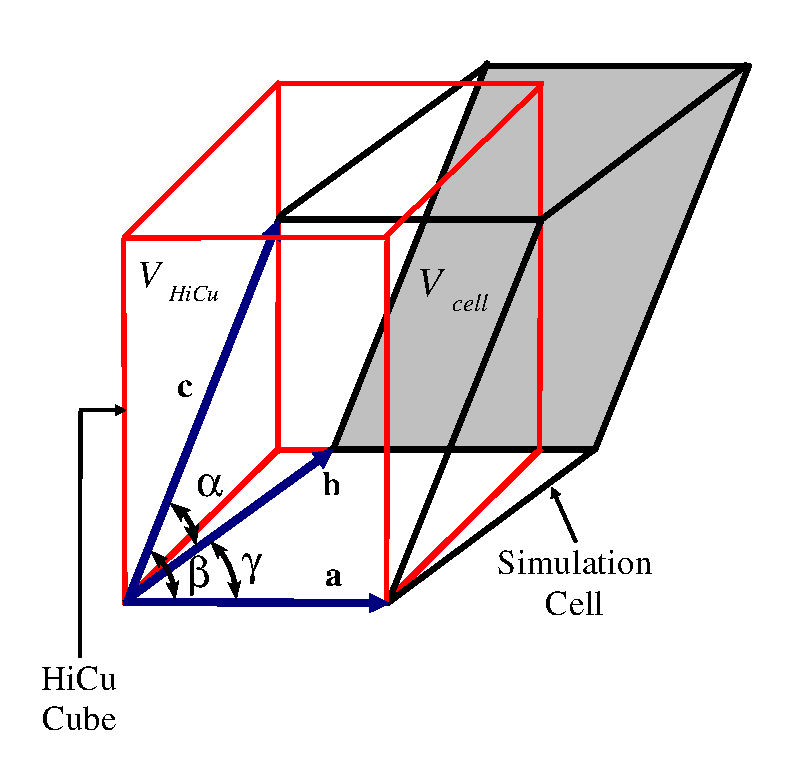
\includegraphics{UnitCell.eps} \par}
\end{figure}



\begin{figure}

\caption{\label{figure: ReplicateCells} Regions which contribute to the Coulomb
Matrix}

{\centering 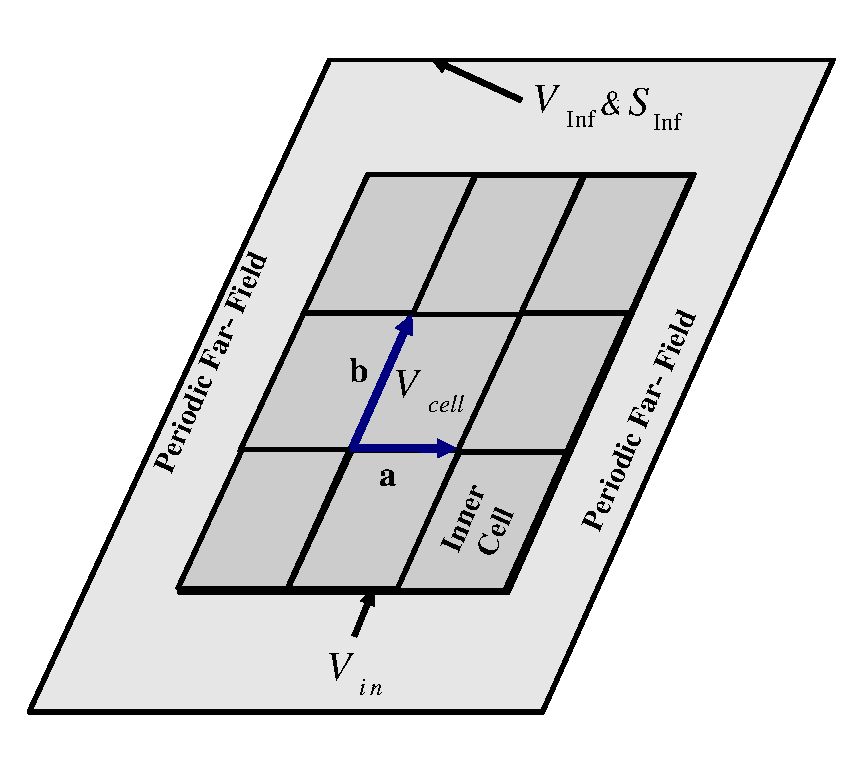
\includegraphics{RepCell.eps} \par}
\end{figure}



\begin{figure}

\caption{\label{figure: ErrorPFF} Error in the Periodic Far Field approximation
with increasing \protect\( \mathbf{L}_{max}\protect \) for two different
inner cell sums for \protect\( 64\protect \) molecules of water.}

{\centering \includegraphics{PFFMultipoles_water.ps} \par}
\end{figure}



\begin{figure}

\caption{\label{figure: Scaling_Matrix_Build} Scaling Results for the matrix
builds \protect\( J_{QCTC}\protect \) and \protect\( K_{xc}\protect \)
for the dense diamond periodic system for the basis set STO-3G and
3-21G.}

\includegraphics{Timing_sto3g_321g.ps} 
\end{figure}



\begin{figure}

\caption{\label{figure: Scaling_Diag} Scaling Results for the Density matix
solver (TRS4) for the dense diamond periodic for the basis set STO-3G
and 3-21G}

system\fbox{\rule[-0.5in]{0pt}{1in}empty figure path} 
\end{figure}

\begin{figure}

\caption{\label{figure:Dense64diamond} Iso-surface potential if a 64 carbon
atom diamond system}

{\centering \fbox{\rule[-0.5in]{0pt}{1in}empty figure path} \par}
\end{figure}



\end{document}
